\subsection{Model and Scene}
The project use a RobomasterS1 robot model, with the addition of four proximity sensors, placed respectively (Figure~\ref{fig:robot_model}):
\begin{itemize}
\item \textbf{Range\_0 (Center-right)}: Primary sensor for orbit distance maintenance during left-side orbital maneuvers. Positioned at the robot's right quadrant with a detection range up to 10 meters.
\item \textbf{Range\_1 (Front-right)}: Primary sensor for initial tower detection and forward-right obstacle detection. Critical for the search phase and collision avoidance.
\item \textbf{Range\_2 (Center-left)}: Secondary sensor utilized during obstacle avoidance protocols, enabling the robot to maintain safe distances from obstacles while navigating around them.
\item \textbf{Range\_3 (Front-left)}: Forward collision prevention sensor that triggers emergency avoidance behaviors when obstacles are detected within critical thresholds.
\end{itemize}
\begin{figure}[H]
    \centering
    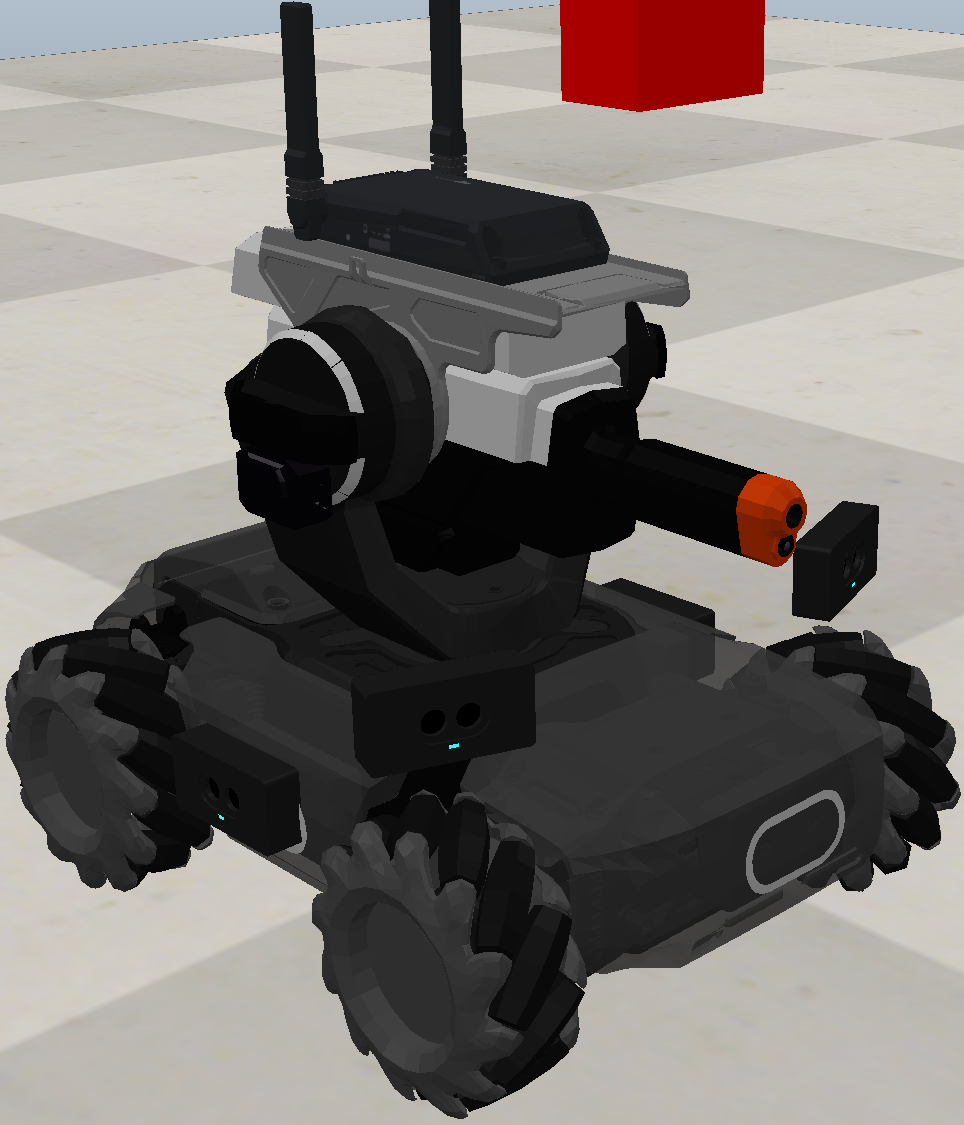
\includegraphics[width=0.2\textwidth]{Images/RobomasterS1_model.png}
    \caption{RobomasterS1 robot model with camera and proximity sensors.}
    \label{fig:robot_model}
\end{figure}
The robot is equipped with a camera (\texttt{/rm0/camera/image\_color}) used for visual processing tasks, such as weak-spot detection and tower identification.\\
The scene is constructed with a 3D model of the RobomasterS1 robot placed in the center of a flat terrain. The environment includes four towers, each colored in red to indicate that they are active and can be targeted. The towers are positioned at the corners of the scene (\text{ADD SOME OTHER DETAILS ABOUT THE SCENE}).\\
\textbf{ADD A PICTURE OF THE SCENE HERE.}\\